\subsection{Image Information Retrieval}
\label{sec:image_information_retrieval}

We want to build a system like this:
\newline
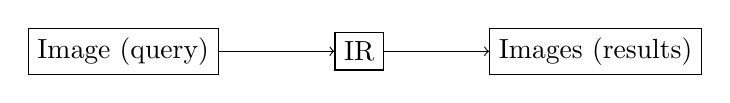
\begin{tikzpicture}
    \node[draw] (input) {Image (query)};
    \node[draw, rectangle, right of=input, node distance=3cm] (ir) {IR};
    \node[draw, right of=ir, node distance=3cm] (output) {Images (results)};
    \draw[->] (input) -- (ir);
    \draw[->] (ir) -- (output);
\end{tikzpicture}
\newline
We want a feature description system that is:
\begin{itemize}
    \item Translation invariant
    \item Rotation invariant
    \item Intensity invariant
    \item Scale invariant
\end{itemize}

A small portion of an image is called a \textbf{patch}.
We want to implement a pipeline that works like this:

% image -> feature detection -> feature description -> feature matching

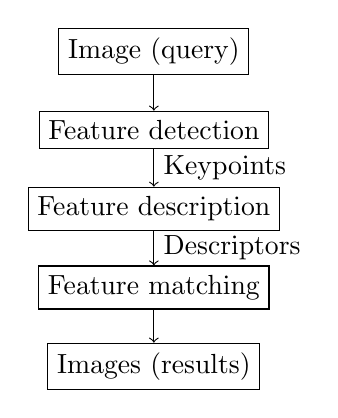
\begin{tikzpicture}
    \node[draw] (input) {Image (query)};
    \node[draw, rectangle, below of=input, node distance=1cm] (fd) {Feature detection};
    \node[draw, rectangle, below of=fd, node distance=1cm] (fdesc) {Feature description};
    \node[draw, rectangle, below of=fdesc, node distance=1cm] (fmatch) {Feature matching};
    \node[draw, below of=fmatch, node distance=1cm] (output) {Images (results)};
    \draw[->] (input) -- (fd);
    \draw[->] (fd) -- node[right] {Keypoints} (fdesc);
    \draw[->] (fdesc) -- node[right] {Descriptors} (fmatch);
    \draw[->] (fmatch) -- (output);
\end{tikzpicture}

\subsubsection{Feature detection}
\label{sec:feature_detection}

We want to detect points of interest (\textbf{keypoints}) in an image.
If we were to detect edges, we would have a problem because them are not descriptive enough.
If we were to detect corners, we would have a problem because they are not scale invariant.
We have to detect \textbf{blobs}.
A \textbf{blob} is a circular flat region of an image.

We can detect a simple blob using the \textbf{LoG} operator.
Depending on the $\sigma$ we choose, we can detect blobs of different sizes.
We normalize the LoG operator to remove the difference in scale depending on the $\sigma$ we choose.
Thus obtaining the \textbf{NLoG} operator $\sigma^2 LoG(x,y,\sigma)$.

Depending on the sigma we choose we detect different size blobs

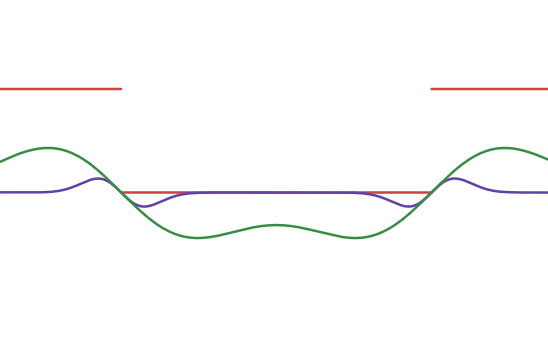
\includegraphics[width=0.3\textwidth]{assets/blob_0.png}
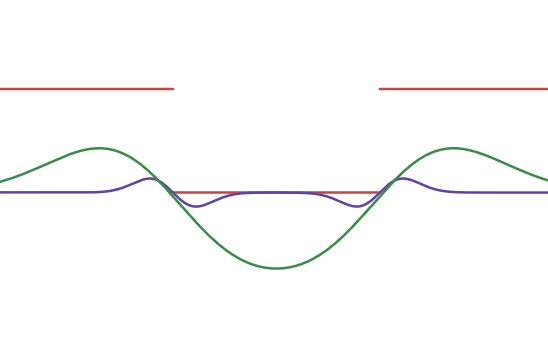
\includegraphics[width=0.3\textwidth]{assets/blob_1.png}
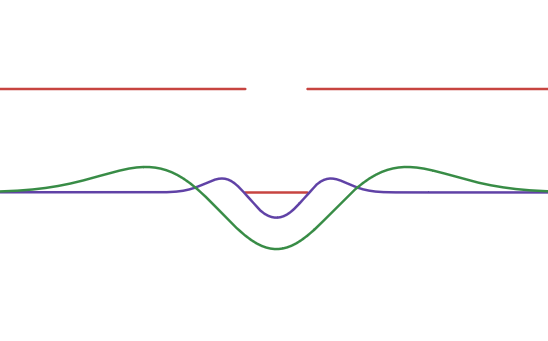
\includegraphics[width=0.3\textwidth]{assets/blob_2.png}

To obtain a description of blobs of each size we must check with different sigmas.
We use many different sigmas close to each other and we obtain a \textbf{scale space}.
The scale space can be expressed like this:
\[
    G[x,y,\sigma] \overset{\Delta}{=} (g[x,y,\sigma_1]*f[x,y], \dots, g[x,y,\sigma_n]*f[x,y])
\]
Usually $\sigma_i=s^i\sigma_1\text{ for }i=2,\dots,n$. Usually $\sigma_1=1.6$.
Usually $s$ is chosens such that $\sigma$ doubles every 2 steps. The number of steps
needed to double $\sigma$ is called octave.

Given a gaussian scale space representation $G[x,y,\sigma]$ the coordinates\\ $x^*,y^*,\sigma^*$ 
of its local minima correspond to keypoints $x^*,y^*$, $\sigma^*$ is called caracteristic scale.
How do we compute keypoints? Using the \textbf{NLoG} operator.
\[
    g_\sigma[x,y,\sigma] = \sigma\nabla^2g[x,y,\sigma] = \sigma LoG[x,y,\sigma]
\]

We want to find $\text{min}G[x,y,\sigma]$.
We will never use the LoG, because the cost is 4 1D convolutions.
If we compute the derivative of a gaussian filter w.r.t. $\sigma$ with the Taylor approximation
up to a factor, we get the following:
\[
    g_\sigma[x,y,\rho\sigma]-g[x,y,\sigma] \approx (\rho-1)NLoG[x,y,\sigma]
\]
This is a new operator called \textbf{Difference of Gaussians} (DoG).
We see that the difference between $g[x,y,\sigma_i]*f[x,y]$ and $g[x,y,\sigma_{i+1}]*f[x,y]$
is approximately $(s-1)$ times the NLoG operator.

We can easily define the DoG representation. 
If we have $G[x,y,\sigma]$ we define 
$D[x,y,\sigma] \overset{\Delta}{=} G[x,y,\sigma_{i+1}]-G[x,y,\sigma_i]\text{ for }0<i<n$
We want to find the local minima of the DoG representation, this is done by

